\documentclass[main.tex]{subfiles}
\begin{document}
\onlyinsubfile{\mainmatter{}}

\chapter{Sealed Closures} \label{ch:cls}
The preceding chapter introduces sealed objects, objects whose state can only be accessed via dedicated methods. This chapter presents an application of sealed objects, a new feature we call \emph{sealed closures}.

\Cref{sct:cls-trad} describes closures and set outs the problems associated with traditional implementations of closures. \Cref{sct:cls-sealed} then presents a sealed object-based solution and a new \g{il}. Finally, \cref{sct:cls-eval} lists the changes in the compiler and evaluates the nanopass approach's impact on the codebase.

\section{Traditional Closures} \label{sct:cls-trad}
A \textbf{closure} is a function that can use the environment\footnote{An environment, and more specifically a \emph{value environment}, can be seen as a mapping from names to values — each definition adds or updates entries in it and the environment is consulted whenever a name is mentioned in the program. That is of course not what happens in an ahead-of-time compiler such as Glyco where the environment consists of registers and memory locations, and the mapping is mostly implemented by the register allocator, but it remains a useful software model nevertheless.} wherein the closure is defined during its operation, i.e., names (variables) valid at the point of the closure definition can also be used in the closure body. The closure is said to \textbf{capture} or \textbf{save} the environment or to \textbf{capture} variables from the \textbf{outer scope}.

The following Swift program uses a closure to print all numbers between 1 and 100, increased by \texttt{offset}.
\begin{swift}
	let offset = 5
	let numbers = (1...100)
		.map { number in number + offset }
	print(numbers)		// 6, 7, 8, 9, 10, …
\end{swift}
The closure takes one parameter \texttt{number} and captures the constant \texttt{offset} from the outer scope. The \texttt{map} method invokes the closure for every number between 1 and 100 inclusive, binding each number to the \texttt{number} parameter. The closure also gets access to \texttt{offset} even though \texttt{map} is not even aware of it.

Closures are usually implemented by pairing a function with an environment. When the pair is invoked, the function is invoked with the environment as a (hidden) parameter. For instance, the following OB program implements a closure \texttt{closure} that takes a single parameter \texttt{n} and captures an environment with a single captured name \texttt{offset}.
\ilfile{Programs/fakecls.ob}

The closure here is implemented as a capability to a record containing a code capability \texttt{function} and a capability \texttt{env} to a record containing fields for each captured value (here just \texttt{offset}). This closure capability (to the function–environment record) can be passed around the program and eventually invoked as shown above — \iil/600/ is in this example the argument to the closure.

The contents of a closure's saved environment are established at the point of closure definition. In most programmer models, the captured value \iil/offset/ from the example above should remain fixed at \iil/5/, which is the value of \iil/offset/ at closure definition. A user of a closure should not be able to execute the closure with a different value for \iil/offset/ than the closure's creator intended. They should only be able to influence the closure's result by providing different arguments, and possibly by influencing any global state that the user has access to and the closure relies on.

In this OB example, it is almost trivially simple to change the value of the \iil/offset/ field, e.g., by writing \iil/do(setField(offset, of: env, to: 10), then: evaluate(…))/.

\section{Sealed Closures} \label{sct:cls-sealed}
The encapsulation problem presented in the previous section is solved in \textbf{sealed closures}, which are closures whose \textbf{captured environment cannot be accessed from outside the closure body}. Sealed closures are presented in a new \g{il} \textbf{CL} (Closures), built on top of OB. CL does not provide any new syntax but instead increases the expressive power provided by λ values, which can now mention names defined outside of the lambda definition. The OB closure example above can now be expressed more elegantly as
\ilfile{Programs/offset.cl}

\paragraph{From CL to OB} The CL to OB \g{nanopass} defines a unique object type for each closure definition and instantiates a single object of that new type. The closure object's state consists of one record entry per captured name. The object is defined with a single method \iil/invoke/ that binds the captured names to the corresponding values in \iil/self/ and then performs the closure body. The above CL program is thus \lowered{} to the OB program
\ilfile{Programs/offset.ob}

\section{Evaluation: Impact on the Codebase} \label{sct:cls-eval}
Similarly to what we did in \cref{sct:ghscc-eval,sct:obj-eval}, we evaluate the impact of the implementation of sealed closures in Glyco by describing the new \gs{il} and changes to existing \gs{il} before quantifying the codebase's growth. The changes to the compiler pipeline are also summarised in \cref{fig:pipeline10}.

\begin{figure}
	\centering
	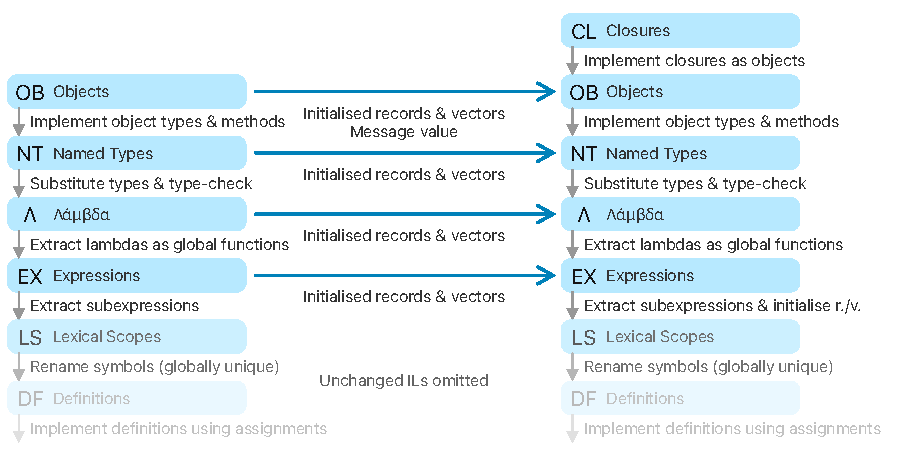
\includegraphics{Images/Pipeline v1.0.pdf}
	\caption{The Glyco 0.3 (left) and 1.0 (right) pipelines and the main differences between them.}
	\label{fig:pipeline10}
\end{figure}

\paragraph{Expressions (EX) through Objects (OB)} The \texttt{record} value is redesigned to accept record entries instead of a record type. The EX to LS \g{nanopass} is updated to initialise the record besides only allocating it, thereby reducing the amount of code needed to create records in higher \gs{il} like OB and CL.

The \texttt{vector} value is redesigned in a similar vein to accept a fill value. The EX to LS \g{nanopass} statically initialises the allocated vector, except when the fill value is \iil/0/ since all allocated buffers are already zero-initialised in the emulator, and should be in a more realistic CHERI-RISC-V runtime environment.

\paragraph{Objects (OB)} The \texttt{message} value is repurposed to \emph{create} a message, i.e., a bound object–method pair, as opposed to \emph{sending} one. Messages are of a new \texttt{message} capability type and can be sent in an \texttt{evaluate} value, which continues to accept normal lambdas. They're represented in NT as a record consisting of an object and method capability, and provide type erasure as required from closures (which are implemented as a unique object type per closure definition).

To reduce the costs of allocating (and initialising) messages, the OB to NT \g{nanopass} recognises the form \iil/evaluate(message(receiver, method), arguments)/ and lowers it by immediately invoking the associated method.

\Gs{init} are redesigned to return an unsealed capability to a record, instead of initialising an already allocated record provided in \iil/self/. The object type no longer declares a state record type, but is now instead inferred from the \g{init}'s result type. In combination with the \texttt{record} value redesign, this reduces the amount of code needed to define an object type.

\paragraph{Closures (CL)} This new \g{il} introduces no new syntax. The CL to OB \g{nanopass} determines captured names and creates unique object types for each closure. As an optimisation, the \g{nanopass} leaves lambdas which do not capture any names as-is.

\paragraph{Codebase growth} The implementation of sealed closures introduces 1 new \g{il} bringing the total in Glyco 1.0 to 23 \gs{il}. Using cloc again, we measured a growth in the codebase from 9360 SLOC in Glyco 0.3 to 10357 SLOC in Glyco 1.0, representing a net growth of $+11\%$. However, as noted before, a significant part of this growth is due to code duplication.

\onlyinsubfile{\glsaddall\printglossaries}
\end{document}
